% file: THTTH-automaton.tex

\documentclass[tikz]{standalone}
\usetikzlibrary{automata, positioning, arrows.meta}

\begin{document}
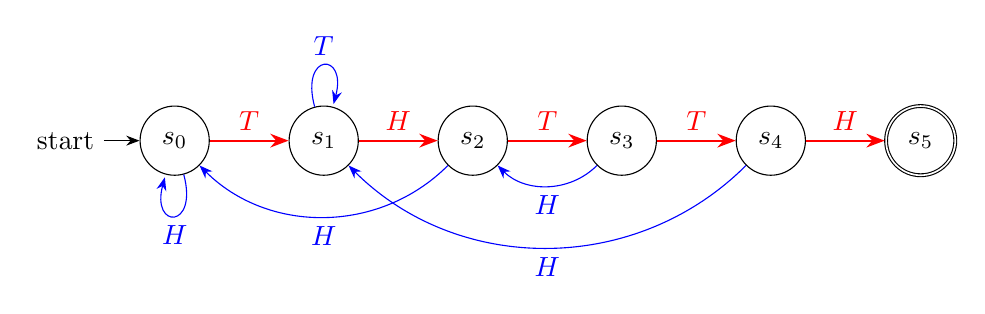
\begin{tikzpicture}[->, >=Stealth, auto, 
  	forward/.style = {thick, red},
	backward/.style = {blue}]
  \node[state, initial] (s0) {$s_0$};
  \node[state, right = of s0] (s1) {$s_1$};
  \node[state, right = of s1] (s2) {$s_2$};
  \node[state, right = of s2] (s3) {$s_3$};
  \node[state, right = of s3] (s4) {$s_4$};
  \node[state, accepting, right = of s4] (s5) {$s_5$};

  \path (s0) edge[forward] node {$T$} (s1)
	     edge[backward, loop below] node {$H$} ()
	(s1) edge[forward] node {$H$} (s2)
	     edge[backward, loop above] node {$T$} (s1)
	(s2) edge[forward] node {$T$} (s3)
	     edge[backward, bend left = 45] node {$H$} (s0)
	(s3) edge[forward] node {$T$} (s4)
	     edge[backward, bend left = 45] node {$H$} (s2)
	(s4) edge[forward] node {$H$} (s5)
	     edge[backward, bend left = 45] node {$H$} (s1);
\end{tikzpicture}
\end{document}
